\documentclass[11pt]{article}
\usepackage[utf8]{inputenc}
\usepackage[T1]{fontenc}
\usepackage[a4paper,margin=20mm]{geometry}
\usepackage{amsmath,amssymb,amsthm}
\usepackage{tikz}
\usepackage{tikz-cd}
\usetikzlibrary{arrows.meta,positioning,fit,backgrounds,calc,shapes.geometric,decorations.pathreplacing}
\usepackage{booktabs}
\usepackage{listings,xcolor}
\usepackage[hidelinks]{hyperref}

% ---------------------------------------------------------------------------
%  Lean listing style (pdflatex-safe: unicode via listings `literate`)
% ---------------------------------------------------------------------------
\definecolor{leanbg}{RGB}{248,248,252}
\definecolor{leankw}{RGB}{140,20,140}
\definecolor{leancm}{RGB}{110,120,130}
\lstdefinestyle{lean}{
  basicstyle=\ttfamily\footnotesize,
  backgroundcolor=\color{leanbg},
  frame=single, framesep=4pt, rulecolor=\color{gray!40},
  breaklines=true, columns=fullflexible, keepspaces=true,
  keywordstyle=\color{leankw}\bfseries,
  commentstyle=\color{leancm}\itshape,
  morecomment=[l]{--},
  morekeywords={theorem,lemma,def,by,namespace,end,variable,open,rw,exact,
    have,intro,induction,with,fun,Prop,Field,Fintype,CharP,set,apply,refine,
    rcases,cases,unfold,simp,ring,ring_nf,grind,linear_combination,omit,in,
    positivity,conv_lhs,show,from},
  literate=
    {∑}{{$\sum$}}1 {∈}{{$\in$}}1 {ℕ}{{$\mathbb{N}$}}1 {→}{{$\to$}}1
    {≠}{{$\neq$}}1 {∨}{{$\vee$}}1 {∧}{{$\wedge$}}1 {∀}{{$\forall$}}1
    {α}{{$\alpha$}}1 {ε}{{$\varepsilon$}}1 {·}{{$\cdot$}}1 {ℓ}{{$\ell$}}1
    {²}{{\textsuperscript{2}}}1 {≡}{{$\equiv$}}1 {𝔽}{{$\mathbb{F}$}}1
    {⟹}{{$\Rightarrow$}}1 {⟨}{{$\langle$}}1 {⟩}{{$\rangle$}}1 {₀}{{$_0$}}1
    {≤}{{$\le$}}1 {↦}{{$\mapsto$}}1 {∣}{{$\mid$}}1 {≥}{{$\ge$}}1
    {←}{{$\leftarrow$}}1 {×}{{$\times$}}1
}
\lstset{style=lean}
\DeclareUnicodeCharacter{2080}{\ensuremath{_0}}
\DeclareUnicodeCharacter{2081}{\ensuremath{_1}}

% ---------------------------------------------------------------------------
%  tikz node styles
% ---------------------------------------------------------------------------
\tikzset{
  found/.style ={draw,rounded corners,align=center,font=\footnotesize,
                 inner sep=3pt,fill=green!9},
  def/.style   ={draw,rounded corners,align=center,font=\footnotesize,
                 inner sep=3pt,fill=gray!10},
  lem/.style   ={draw,rounded corners,align=center,font=\footnotesize,
                 inner sep=3pt,fill=blue!8},
  head/.style  ={draw,rounded corners,align=center,font=\footnotesize\bfseries,
                 inner sep=4pt,fill=orange!18},
  ar/.style    ={-{Stealth[length=2mm]},shorten >=1pt,shorten <=1pt},
  layer/.style ={draw=none,font=\small\bfseries,rotate=90,anchor=center},
}
\newcommand{\lc}[1]{\texttt{#1}}
\newcommand{\Tr}{\operatorname{Tr}}
\newtheorem*{remark}{Remark}

\title{\bfseries From First Principles to the First Step of\\
  Dobbertin's Theorem~1\\[4pt]
  \large A bottom-up account of the \lc{DobbertinStep1} Lean~4 formalisation}
\author{}
\date{}

\begin{document}
\maketitle

\begin{abstract}
We reconstruct, \emph{from the ground up}, the Lean~4 / Mathlib formalisation of
the opening step of the proof of Theorem~1 in H.~Dobbertin, \emph{Kasami Power
Functions, Permutation Polynomials and Cyclic Difference Sets} (NATO Sci.\ Ser.\
C \textbf{542}, 1999, pp.~133--158): the implication \emph{equation~(1)}
$\Rightarrow$ \emph{equation~(2)}.  Starting from the simplest foundational
ingredients (a handful of characteristic-$2$ finite-field facts from Mathlib),
we introduce the definitions, then compose progressively richer lemmas, each
presented in ordinary mathematical notation \emph{beside} its exact Lean
statement, until the two ingredients ---an Artin--Schreier telescoping and the
fact that the trace is a bit--- combine into the headline theorem.  A layered
build diagram, a commutative diagram of the derivation, and dependency graphs
make the compositional structure explicit.
\end{abstract}

\tableofcontents

% ===========================================================================
\section{The target, and the plan}
% ===========================================================================
Fix $F=\mathbb{F}_{2^n}$, a finite field of characteristic~$2$, and integers
$k,k'$ with $k\,k'\equiv 1\pmod n$.  For $c\in F$, Dobbertin's equation~(1)
(cleared of denominators) reads
\begin{equation}
  c\,x^{2^k+1}=\sum_{i=1}^{k'}x^{2^{ik}}+\alpha\,\Tr(x),\qquad \alpha\in\{0,1\},
  \tag{1}
\end{equation}
and its \emph{linearized} consequence, equation~(2), is $\ell(x)=0$ where
\begin{equation}
  \ell(x)=c^{2^k}x^{2^{2k}}+x^{2^k}+c\,x+1 .
  \tag{2}
\end{equation}

\paragraph{Goal.}  Prove, in Lean, that for every nonzero $x$ and every
$\alpha\in\{0,1\}$, \emph{(1) implies (2)}.  In Lean this is one theorem:

\begin{lstlisting}
theorem equation2_of_equation1 {n k k' α : ℕ} (hn : Fintype.card F = 2 ^ n)
    (hkk' : k * k' % n = 1) (hα : α = 0 ∨ α = 1) {c x : F} (hx : x ≠ 0)
    (h : equation1 n k k' α c x) : linearized k c x = 0
\end{lstlisting}

\paragraph{Plan (bottom-up).}  We build the proof in five layers.  Each layer
uses only the layers below it.

\begin{center}
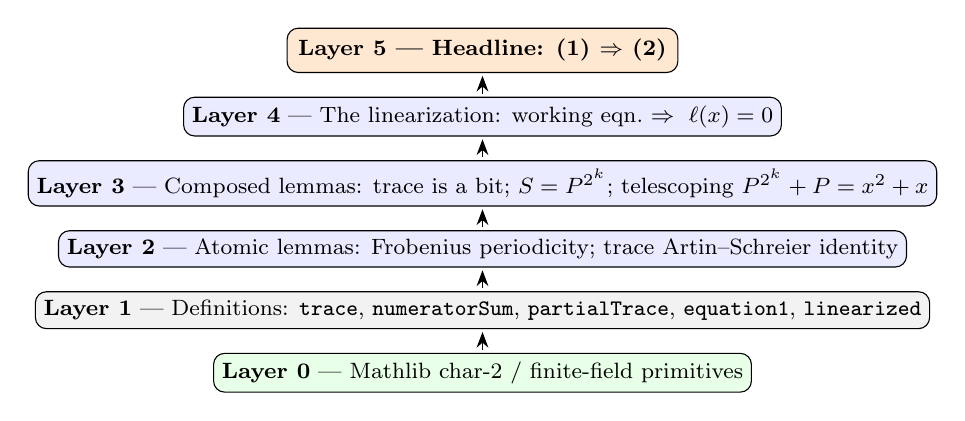
\begin{tikzpicture}[node distance=3mm and 6mm]
\node[found] (L0) {\textbf{Layer 0} — Mathlib char-$2$ / finite-field primitives};
\node[def, above=of L0] (L1) {\textbf{Layer 1} — Definitions: \lc{trace}, \lc{numeratorSum}, \lc{partialTrace}, \lc{equation1}, \lc{linearized}};
\node[lem, above=of L1] (L2) {\textbf{Layer 2} — Atomic lemmas: Frobenius periodicity; trace Artin--Schreier identity};
\node[lem, above=of L2] (L3) {\textbf{Layer 3} — Composed lemmas: trace is a bit; $S=P^{2^k}$; telescoping $P^{2^k}+P=x^2+x$};
\node[lem, above=of L3] (L4) {\textbf{Layer 4} — The linearization: working eqn.\ $\Rightarrow\ \ell(x)=0$};
\node[head, above=of L4] (L5) {\textbf{Layer 5} — Headline: (1) $\Rightarrow$ (2)};
\draw[ar] (L0)--(L1); \draw[ar] (L1)--(L2); \draw[ar] (L2)--(L3);
\draw[ar] (L3)--(L4); \draw[ar] (L4)--(L5);
\end{tikzpicture}
\end{center}

% ===========================================================================
\section{Layer 0 --- the foundational ingredients}
% ===========================================================================
The whole development rests on a small, fixed set of facts about a finite field
$F$ of characteristic~$2$ with $|F|=2^n$.  These are the ``atoms'': everything
else is assembled from them.

\begin{center}\small
\begin{tabular}{@{}lll@{}}
\toprule
\textbf{Fact} & \textbf{Mathematics} & \textbf{Mathlib name}\\
\midrule
Frobenius fixes $F$      & $x^{|F|}=x$                       & \lc{FiniteField.pow\_card}\\
Freshman's dream         & $(a+b)^2=a^2+b^2$                 & \lc{add\_pow\_char}\\
iterated freshman        & $(a+b)^{2^k}=a^{2^k}+b^{2^k}$     & \lc{add\_pow\_char\_pow}\\
sum version              & $(\sum a_i)^{2^k}=\sum a_i^{2^k}$ & \lc{sum\_pow\_char\_pow}\\
$x+x=0$                  & doubling is zero                  & \lc{CharTwo.add\_self\_eq\_zero}\\
$2=0$                    & characteristic two                & \lc{CharTwo.two\_eq\_zero}\\
\bottomrule
\end{tabular}
\end{center}

Two structural consequences of char~$2$ drive every cancellation below:
\[
  a+a=0 \quad\text{(``things that appear twice vanish'')},\qquad
  (a+b)^{2^k}=a^{2^k}+b^{2^k}\quad\text{(``$2^k$-th power is additive'')}.
\]
The Lean context carrying these is simply
\begin{lstlisting}
variable {F : Type*} [Field F] [Fintype F] [CharP F 2]
\end{lstlisting}

% ===========================================================================
\section{Layer 1 --- the definitions}
% ===========================================================================
Five definitions turn the paper's symbols into Lean objects
(\lc{DobbertinStep1/Defs.lean}).  Nothing here is proved yet; these are the
nouns of the story.

\begin{center}\small
\begin{tabular}{@{}lll@{}}
\toprule
\textbf{Symbol} & \textbf{Meaning} & \textbf{Lean}\\
\midrule
$\Tr(x)=\sum_{i<n}x^{2^i}$        & absolute trace        & \lc{trace n x}\\
$S(x)=\sum_{i=1}^{k'}x^{2^{ik}}$  & numerator sum         & \lc{numeratorSum k k' x}\\
$P(x)=\sum_{j<k'}x^{2^{jk}}$      & partial trace         & \lc{partialTrace k k' x}\\
eqn.~(1)                          & cleared equation      & \lc{equation1 n k k' $\alpha$ c x}\\
$\ell(x)$                         & linearized polynomial & \lc{linearized k c x}\\
\bottomrule
\end{tabular}
\end{center}

\begin{lstlisting}
def trace (n : ℕ) (x : F) : F := ∑ i ∈ range n, x ^ (2 ^ i)

def numeratorSum (k k' : ℕ) (x : F) : F := ∑ i ∈ Icc 1 k', x ^ (2 ^ (i * k))

def partialTrace (k k' : ℕ) (x : F) : F := ∑ j ∈ range k', x ^ (2 ^ (j * k))

def equation1 (n k k' α : ℕ) (c x : F) : Prop :=
  c * x ^ (2 ^ k + 1) = numeratorSum k k' x + (α : F) * trace n x

def linearized (k : ℕ) (c x : F) : F :=
  c ^ (2 ^ k) * x ^ (2 ^ (2 * k)) + x ^ (2 ^ k) + c * x + 1
\end{lstlisting}

The key design choice is the pair $S$ vs.\ $P$.  The right-hand side of~(1) is
$S(x)=\sum_{i=1}^{k'}x^{2^{ik}}$; the \emph{partial trace}
$P(x)=\sum_{j=0}^{k'-1}x^{2^{jk}}$ is the same sum shifted down by one Frobenius
step.  Their relationship, $S=P^{2^k}$, is exactly what lets us ``add the
$2^k$-th power of~(1) to itself''.

% ===========================================================================
\section{Layer 2 --- atomic lemmas}
% ===========================================================================
These are the first proved facts; each rests \emph{directly} on Layer~0.

\subsection{Frobenius periodicity}
\label{sec:frob}
Because $x^{2^n}=x^{|F|}=x$, the exponent $2^r$ only matters modulo~$n$.

\[
  \boxed{\;x^{2^r}=x^{2^{\,r\bmod n}}\;}
  \qquad\text{(\lc{pow\_two\_pow\_mod})}
\]

\begin{lstlisting}
lemma pow_two_pow_mod {n : ℕ} (hn : Fintype.card F = 2 ^ n) (x : F) (r : ℕ) :
    x ^ (2 ^ r) = x ^ (2 ^ (r % n)) := by
  conv_lhs => rw [show r = n * (r / n) + r % n from (Nat.div_add_mod r n).symm,
    pow_add, pow_mul]
  have step : ∀ j : ℕ, x ^ (2 ^ (n * j)) = x := by
    intro j
    induction j with
    | zero => simp
    | succ j ih => rw [Nat.mul_succ, pow_add, pow_mul, ← hn, FiniteField.pow_card, ih]
  rw [step]
\end{lstlisting}

\noindent\emph{Idea.}  Write $r=n\lfloor r/n\rfloor+(r\bmod n)$; the first part
contributes $x^{2^{n\cdot j}}=x$ by iterating $x^{2^n}=x$ ($j$ times).

\subsection{The trace's Artin--Schreier identity}
Squaring is additive, so squaring the telescoping sum $\Tr(x)=\sum_{i<n}x^{2^i}$
collapses everything except the two ends:
\[
  \boxed{\;\Tr(x)^2+\Tr(x)=x^{2^n}+x\;}
  \qquad\text{(\lc{trace\_sq\_add\_self})}.
\]

\begin{lstlisting}
lemma trace_sq_add_self (n : ℕ) (x : F) :
    trace n x ^ 2 + trace n x = x ^ (2 ^ n) + x := by
  induction n with
  | zero => simp [trace, CharTwo.add_self_eq_zero]
  | succ n ih => ...  -- peel off the top summand, use (a+b)²=a²+b², cancel in char 2
\end{lstlisting}

\noindent\emph{Idea.}  Induct on $n$.  The step splits
$\Tr_{n+1}=\Tr_n+x^{2^n}$; squaring is additive, so
$\Tr_{n+1}^2=\Tr_n^2+x^{2^{n+1}}$; the induction hypothesis and a char-$2$
cancellation of the repeated $x^{2^n}$ finish it.  (This lemma needs no
finiteness of $F$ --- it is pure characteristic-$2$ algebra, hence
\lc{omit [Fintype F]}.)

% ===========================================================================
\section{Layer 3 --- composed lemmas}
% ===========================================================================
Now the two independent strands of the proof appear: the \emph{trace bit} and
the \emph{telescoping}.

\subsection{Strand A: the trace is a bit}
Specialising $x^{2^n}=x$ in the Artin--Schreier identity gives idempotence, and
idempotence over a field forces $\Tr(x)\in\{0,1\}$.
\[
  \Tr(x)^2=\Tr(x)
  \;\underset{\Tr(\Tr-1)=0}{\Longrightarrow}\;
  \boxed{\;\Tr(x)=0\ \vee\ \Tr(x)=1\;}
\]
\begin{lstlisting}
lemma trace_sq {n : ℕ} (hn : Fintype.card F = 2 ^ n) (x : F) :
    trace n x ^ 2 = trace n x
lemma trace_eq_zero_or_one {n : ℕ} (hn : Fintype.card F = 2 ^ n) (x : F) :
    trace n x = 0 ∨ trace n x = 1
\end{lstlisting}
This is the ``$=0$ or $1$'' input Dobbertin uses: it lets us collapse the term
$\alpha\,\Tr(x)$ into a single bit $\varepsilon\in\{0,1\}$.

\subsection{Strand B: telescoping the partial trace}
First, the shift relation ($S$ is the Frobenius image of $P$):
\[
  S(x)=P(x)^{2^k}\qquad\text{(\lc{numeratorSum\_eq\_partialTrace\_frob})}.
\]
\begin{lstlisting}
lemma numeratorSum_eq_partialTrace_frob (k k' : ℕ) (x : F) :
    numeratorSum k k' x = partialTrace k k' x ^ (2 ^ k)
\end{lstlisting}
Then the char-$2$ telescoping of the linearized polynomial $P$: adding
$P^{2^k}$ to $P$ makes every interior term appear twice, leaving only the ends,
\[
  P(x)^{2^k}+P(x)=x^{2^{k'k}}+x
  \qquad\text{(\lc{partialTrace\_telescope\_raw})}.
\]
\begin{lstlisting}
lemma partialTrace_telescope_raw (k k' : ℕ) (x : F) :
    partialTrace k k' x ^ (2 ^ k) + partialTrace k k' x
      = x ^ (2 ^ (k' * k)) + x
\end{lstlisting}
Finally, feed in Frobenius periodicity (Section~\ref{sec:frob}): since
$k\,k'\equiv1\pmod n$, the exponent $2^{k'k}$ collapses to $2^1=2$, giving the
Artin--Schreier form
\[
  \boxed{\;P(x)^{2^k}+P(x)=x^2+x\;}
  \qquad\text{(\lc{partialTrace\_telescope})}.
\]
\begin{lstlisting}
lemma partialTrace_telescope {n k k' : ℕ} (hn : Fintype.card F = 2 ^ n)
    (hkk' : k * k' % n = 1) (x : F) :
    partialTrace k k' x ^ (2 ^ k) + partialTrace k k' x = x ^ 2 + x := by
  rw [partialTrace_telescope_raw]
  have : x ^ (2 ^ (k' * k)) = x ^ 2 := by
    rw [pow_two_pow_mod hn x (k' * k), Nat.mul_comm k' k, hkk', pow_one]
  rw [this]
\end{lstlisting}

% ===========================================================================
\section{Layer 4 --- the linearization}
% ===========================================================================
This is the algebraic heart: ``adding the $2^k$-th power of the equation to
itself''.  Assume $x\neq0$ and that $x$ solves the \emph{working} form of~(1)
with the trace term already collapsed to a bit $\varepsilon\in\{0,1\}$:
\[
  S(x)+\varepsilon=c\,x^{2^k+1}. \tag{$1'$}
\]

\begin{lstlisting}
lemma linearized_eq_zero_of_solution {n k k' : ℕ} (hn : Fintype.card F = 2 ^ n)
    (hkk' : k * k' % n = 1) {ε : F} (hε : ε = 0 ∨ ε = 1) {c x : F} (hx : x ≠ 0)
    (hsol : numeratorSum k k' x + ε = c * x ^ (2 ^ k + 1)) :
    linearized k c x = 0
\end{lstlisting}

\paragraph{Derivation.}  Write $S=P^{2^k}$ and $T=P^{2^k}+P=x^2+x$.

\begin{enumerate}\itemsep2pt
\item \textbf{Solve $(1')$ for $P$.}  From $T=x^2+x$ and
      $P^{2^k}=S=c\,x^{2^k+1}+\varepsilon$,
      \[ P=(x^2+x)+c\,x^{2^k+1}+\varepsilon. \]
\item \textbf{Raise to the $2^k$-th power} (additive, and
      $\varepsilon^{2^k}=\varepsilon$ since $\varepsilon$ is a bit):
      \[ S=P^{2^k}=(x^2)^{2^k}+x^{2^k}+\bigl(c\,x^{2^k+1}\bigr)^{2^k}+\varepsilon. \]
\item \textbf{Cancel $\varepsilon$} against $(1')$ to reach the core relation
      between powers of $x$:
      \[ c\,x^{2^k+1}=(x^2)^{2^k}+x^{2^k}+\bigl(c\,x^{2^k+1}\bigr)^{2^k}. \]
\item \textbf{Reduce the exponents.}  Using $(x^2)^{2^k}=x^{2^k}\!\cdot x^{2^k}$
      and $(2^k+1)2^k=2^{2k}+2^k$,
      \[ \bigl(c\,x^{2^k+1}\bigr)^{2^k}=c^{2^k}\bigl(x^{2^{2k}}\!\cdot x^{2^k}\bigr). \]
\item \textbf{Divide by $x^{2^k}\neq0$.}  Every surviving term carries a factor
      $x^{2^k}$; cancelling it turns the core relation into
      $c\,x=x^{2^k}+1+c^{2^k}x^{2^{2k}}$, i.e.
      \[ \ell(x)=c^{2^k}x^{2^{2k}}+x^{2^k}+c\,x+1=0. \qquad\blacksquare \]
\end{enumerate}

\noindent The five steps correspond one-to-one to the \lc{have}s in the Lean
proof (\lc{hP\_sub}, \lc{hS\_pow}, \lc{h\_core}, \lc{e1}/\lc{e2}, the final
\lc{mul\_left\_cancel₀}); the character-$2$ cancellations are discharged by
\lc{grind +ring} and \lc{linear\_combination}.

\begin{remark}[why $x\neq0$ is essential]
At $x=0$ the cleared equation~(1) reads $0=0$ and holds \emph{vacuously}, yet
$\ell(0)=1\neq0$.  Step~5 divides by $x^{2^k}$, which is exactly where $x=0$ is
excluded --- faithfully matching Dobbertin, who works with the nonzero solutions.
\end{remark}

% ===========================================================================
\section{Layer 5 --- the headline}
% ===========================================================================
The top theorem simply glues the two strands: use \lc{trace\_eq\_zero\_or\_one}
(Strand~A) to collapse $\alpha\,\Tr(x)$ to a bit $\varepsilon$, then apply
\lc{linearized\_eq\_zero\_of\_solution} (Strand~B $+$ Layer~4).

\begin{lstlisting}
theorem equation2_of_equation1 {n k k' α : ℕ} (hn : Fintype.card F = 2 ^ n)
    (hkk' : k * k' % n = 1) (hα : α = 0 ∨ α = 1) {c x : F} (hx : x ≠ 0)
    (h : equation1 n k k' α c x) :
    linearized k c x = 0 := by
  have hbit : (α : F) * trace n x = 0 ∨ (α : F) * trace n x = 1 := by
    have hαcast : (α : F) = 0 ∨ (α : F) = 1 := by rcases hα with rfl | rfl <;> simp
    rcases hαcast with h0 | h1
    · exact Or.inl (by rw [h0, zero_mul])
    · rw [h1, one_mul]; exact trace_eq_zero_or_one hn x
  exact linearized_eq_zero_of_solution hn hkk' hbit hx h.symm
\end{lstlisting}

% ===========================================================================
\section{The derivation as a commutative diagram}
% ===========================================================================
Writing $\varepsilon=\alpha\,\Tr(x)\in\{0,1\}$, the two inputs (trace bit and
telescoping) combine into the single implication:
\begin{center}
\begin{tikzcd}[column sep=huge, row sep=large]
\boxed{\;c\,x^{2^k+1}=S(x)+\alpha\,\Tr(x)\;}
  \arrow[r, "\text{\lc{trace\_eq\_zero\_or\_one}}"]
  \arrow[d, swap, "\text{collapse }\alpha\Tr\text{ to a bit}"]
& S(x)+\varepsilon=c\,x^{2^k+1},\ \varepsilon\in\{0,1\}
  \arrow[d, "\substack{S=P^{2^k}\\ P^{2^k}+P=x^2+x}"]\\
\boxed{\;\ell(x)=0\;}
& P=(x^2+x)+c\,x^{2^k+1}+\varepsilon
  \arrow[l, "\substack{\text{raise to }2^k,\ \varepsilon^{2^k}=\varepsilon\\ \text{divide by }x^{2^k}\neq0}"]
\end{tikzcd}
\end{center}

% ===========================================================================
\section{The full compositional build}
% ===========================================================================
The diagram below shows \emph{everything at once}: how each declaration is
assembled from the ones beneath it, organised by the five layers.  An edge
$A\to B$ means ``$A$ is built using $B$''.  The two vertical strands (trace bit
on the right, telescoping on the left) meet only at the headline.

\begin{center}
\resizebox{\textwidth}{!}{%
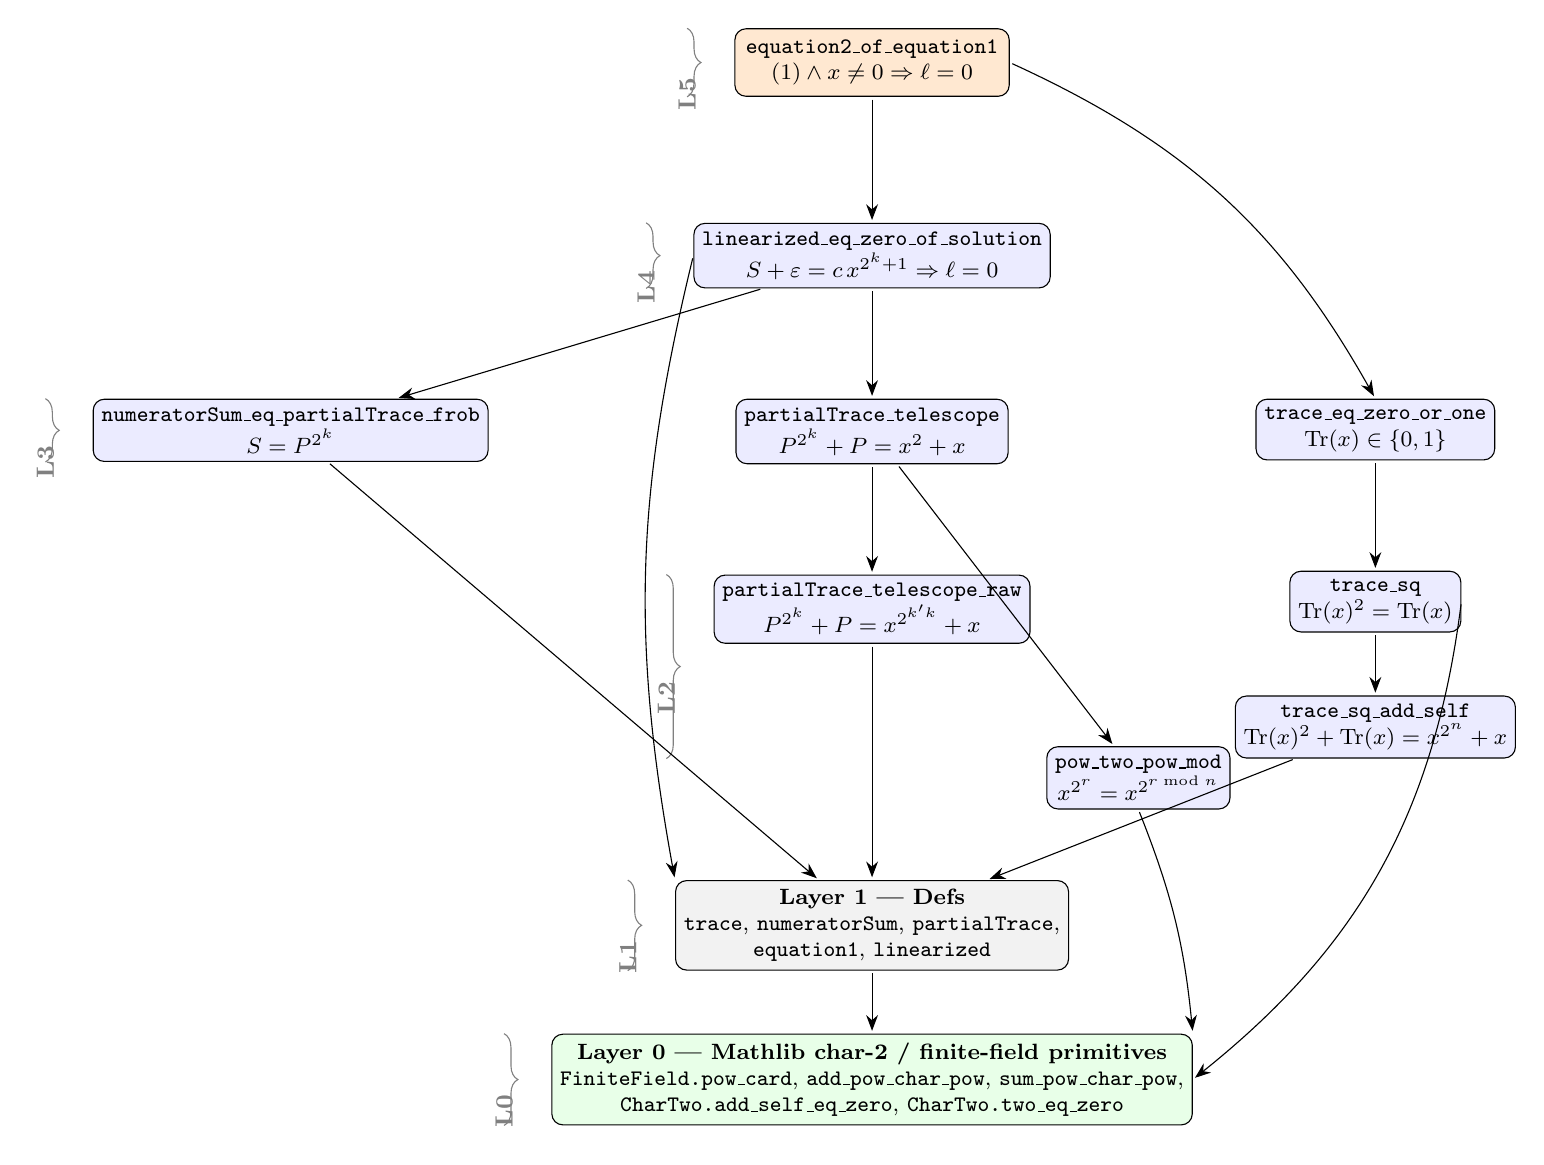
\begin{tikzpicture}[node distance=9mm and 10mm]
% Layer 5
\node[head] (H) {\lc{equation2\_of\_equation1}\\ $(1)\wedge x\neq0\Rightarrow \ell=0$};
% Layer 4
\node[lem,below=16mm of H] (LIN) {\lc{linearized\_eq\_zero\_of\_solution}\\ $S+\varepsilon=c\,x^{2^k+1}\Rightarrow \ell=0$};
% Layer 3 : two strands
\node[lem,below left=14mm and 26mm of LIN] (SEQ) {\lc{numeratorSum\_eq\_partialTrace\_frob}\\ $S=P^{2^k}$};
\node[lem,below=14mm of LIN] (TEL) {\lc{partialTrace\_telescope}\\ $P^{2^k}+P=x^2+x$};
\node[lem,below right=14mm and 26mm of LIN] (TB) {\lc{trace\_eq\_zero\_or\_one}\\ $\Tr(x)\in\{0,1\}$};
% Layer 2
\node[lem,below=14mm of TEL] (RAW) {\lc{partialTrace\_telescope\_raw}\\ $P^{2^k}+P=x^{2^{k'k}}+x$};
\node[lem,below right=13mm and 2mm of RAW] (FROB) {\lc{pow\_two\_pow\_mod}\\ $x^{2^r}=x^{2^{r\bmod n}}$};
\node[lem,below=14mm of TB] (TSQ) {\lc{trace\_sq}\\ $\Tr(x)^2=\Tr(x)$};
\node[lem,below=8mm of TSQ] (TSAS) {\lc{trace\_sq\_add\_self}\\ $\Tr(x)^2+\Tr(x)=x^{2^n}+x$};
% Layer 1
\node[def,below=30mm of RAW] (DEFS) {\textbf{Layer 1 — Defs}\\ \lc{trace}, \lc{numeratorSum}, \lc{partialTrace},\\ \lc{equation1}, \lc{linearized}};
% Layer 0
\node[found,below=8mm of DEFS] (M) {\textbf{Layer 0 — Mathlib char-2 / finite-field primitives}\\ \lc{FiniteField.pow\_card}, \lc{add\_pow\_char\_pow}, \lc{sum\_pow\_char\_pow},\\ \lc{CharTwo.add\_self\_eq\_zero}, \lc{CharTwo.two\_eq\_zero}};
% edges
\draw[ar] (H) -- (LIN);
\draw[ar] (H.east) to[bend left=18] (TB.north);
\draw[ar] (LIN) -- (SEQ);
\draw[ar] (LIN) -- (TEL);
\draw[ar] (TEL) -- (RAW);
\draw[ar] (TEL) -- (FROB);
\draw[ar] (TB) -- (TSQ);
\draw[ar] (TSQ) -- (TSAS);
\draw[ar] (SEQ) -- (DEFS);
\draw[ar] (RAW) -- (DEFS);
\draw[ar] (TSAS) -- (DEFS);
\draw[ar] (LIN.west) to[bend right=12] (DEFS.north west);
\draw[ar] (FROB.south) to[bend left=8] (M.north east);
\draw[ar] (TSQ.east) to[bend left=22] (M.east);
\draw[ar] (DEFS) -- (M);
% layer brackets
\begin{scope}[on background layer]
\draw[decorate,decoration={brace,amplitude=5pt},gray]
  ([xshift=-6mm]H.north west) -- ([xshift=-6mm]H.south west) node[layer,midway,xshift=-4mm]{L5};
\draw[decorate,decoration={brace,amplitude=5pt},gray]
  ([xshift=-6mm]LIN.north west) -- ([xshift=-6mm]LIN.south west) node[layer,midway,xshift=-4mm]{L4};
\draw[decorate,decoration={brace,amplitude=5pt},gray]
  ([xshift=-6mm]SEQ.north west) -- ([xshift=-6mm]SEQ.south west) node[layer,midway,xshift=-4mm]{L3};
\draw[decorate,decoration={brace,amplitude=5pt},gray]
  ([xshift=-6mm]RAW.north west) -- ([xshift=-6mm]TSAS.south -| RAW.west) node[layer,midway,xshift=-4mm]{L2};
\draw[decorate,decoration={brace,amplitude=5pt},gray]
  ([xshift=-6mm]DEFS.north west) -- ([xshift=-6mm]DEFS.south west) node[layer,midway,xshift=-4mm]{L1};
\draw[decorate,decoration={brace,amplitude=5pt},gray]
  ([xshift=-6mm]M.north west) -- ([xshift=-6mm]M.south west) node[layer,midway,xshift=-4mm]{L0};
\end{scope}
\end{tikzpicture}}
\end{center}

% ===========================================================================
\section{Module structure and the proof space}
% ===========================================================================
The declarations live in six modules over a common Mathlib base.  The
\emph{directed} dependency DAG (left) is transcribed \emph{verbatim} into a Lean
relation \lc{dep}; the induced \emph{undirected} \lc{SimpleGraph} \lc{depGraph}
(right) is proved \textbf{connected} in \lc{DobbertinStep1/ProofSpace.lean},
certifying that no component is orphaned.

\begin{center}
\begin{minipage}[c]{0.46\textwidth}\centering
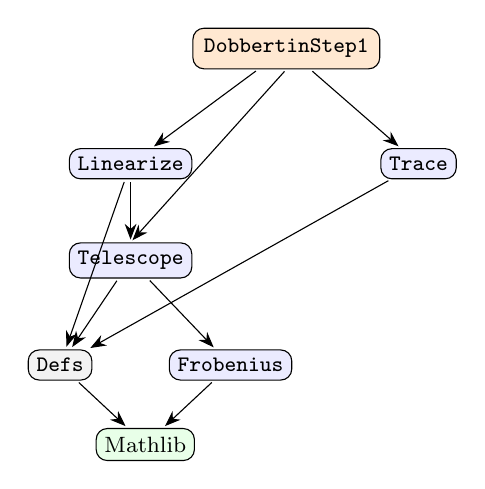
\begin{tikzpicture}[node distance=8mm and 8mm]
\node[head] (S1) {\lc{DobbertinStep1}};
\node[lem,below left=10mm and 0mm of S1] (LIN) {\lc{Linearize}};
\node[lem,below right=10mm and 0mm of S1] (TR) {\lc{Trace}};
\node[lem,below=of LIN] (TEL) {\lc{Telescope}};
\node[def,below left=9mm and -3mm of TEL] (DE) {\lc{Defs}};
\node[lem,below right=9mm and -3mm of TEL] (FR) {\lc{Frobenius}};
\node[found,below=8mm of $(DE)!0.5!(FR)$] (M) {Mathlib};
\draw[ar] (S1)--(LIN); \draw[ar] (S1)--(TR); \draw[ar] (S1.south)--(TEL.north);
\draw[ar] (LIN)--(TEL); \draw[ar] (LIN)--(DE); \draw[ar] (TR)--(DE);
\draw[ar] (TEL)--(DE); \draw[ar] (TEL)--(FR);
\draw[ar] (DE)--(M); \draw[ar] (FR)--(M);
\end{tikzpicture}\\[2pt]
{\footnotesize directed DAG $=$ Lean \lc{dep}}
\end{minipage}\hfill
\begin{minipage}[c]{0.5\textwidth}\centering
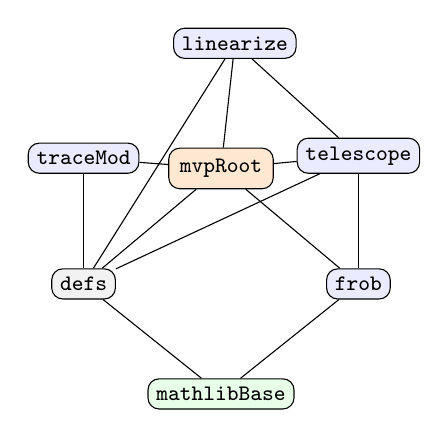
\begin{tikzpicture}[node distance=9mm and 10mm,every edge/.style={draw,thick}]
\node[found] (M) {\lc{mathlibBase}};
\node[def,above left=10mm and 4mm of M] (DE) {\lc{defs}};
\node[lem,above right=10mm and 4mm of M] (FR) {\lc{frob}};
\node[lem,above=12mm of DE] (TR) {\lc{traceMod}};
\node[lem,above=12mm of FR] (TEL) {\lc{telescope}};
\node[lem,above left=10mm and 0mm of TEL] (LIN) {\lc{linearize}};
\node[head,above=24mm of M] (S1) {\lc{mvpRoot}};
\draw (DE)--(M); \draw (FR)--(M);
\draw (TR)--(DE); \draw (TEL)--(DE); \draw (TEL)--(FR);
\draw (LIN)--(DE); \draw (LIN)--(TEL);
\draw (S1)--(DE); \draw (S1)--(FR); \draw (S1)--(TR);
\draw (S1)--(TEL); \draw (S1)--(LIN);
\end{tikzpicture}\\[2pt]
{\footnotesize undirected \lc{depGraph} $=$ \lc{SimpleGraph.fromRel dep}}
\end{minipage}
\end{center}

\begin{lstlisting}
theorem depGraph_connected : depGraph.Connected
\end{lstlisting}

% ===========================================================================
\section*{Soundness}
% ===========================================================================
\addcontentsline{toc}{section}{Soundness}
Every declaration in \lc{DobbertinStep1} is \lc{sorry}-free; \lc{lake build}
succeeds, and the headline \lc{equation2\_of\_equation1} depends only on the
standard axioms \lc{propext}, \lc{Classical.choice}, \lc{Quot.sound}.

\end{document}
